\documentclass{beamer}
\mode<presentation>
{
  \usetheme{default}      % or try Darmstadt, Madrid, Warsaw, ...
  \usecolortheme{default} % or try albatross, beaver, crane, ...
  \usefonttheme{default}  % or try serif, structurebold, ...
  \setbeamertemplate{navigation symbols}{}
  \setbeamertemplate{caption}[numbered]
} 


\usepackage[english]{babel}
\usepackage[utf8x]{inputenc}
\usepackage{scrextend}
\usepackage{graphicx}
\usepackage{booktabs}
\usepackage{adjustbox}
\usepackage{marvosym}

\graphicspath{ {images/} }

\setbeamertemplate{footline}{
\hfill
\insertframenumber{}/
\inserttotalframenumber
}

\title[Pres]{Methods and Tools for the Analysis of Legacy Software Systems}
\author{Stana Adelina Diana}
\institute{Computer Science and Engineering Department\\
"Politehnica" University of Timisoara}
\date{2019}

\begin{document}

\begin{frame}
  \titlepage
\end{frame}

%%%%%%%%%%%%%%%%%%%%%%%%%%%%%%%%%%%%%%%%%%
\section{Presentation of the research topic}
 \begin{frame}
\frametitle{Presentation of the research topic}
 The thesis will develop methods for the analysis of software systems
 using historical information from the versioning systems\footnote{Versioning systems keep track of every change to a file over time so early versions can be restored and used by software teams.}. 
\end{frame}

%%%%%%%%%%%%%%%%%%%%%%%%%%%%%%%%%%%%%%%%%%

 \begin{frame}
\frametitle{Structural dependencies}
\begin{block}{Definition}
Structural dependencies are the result of \it{source code analysis} and can be extracted from : members, call parameters, local variables. 
\end{block}

\begin{center}
     \begin{figure}
	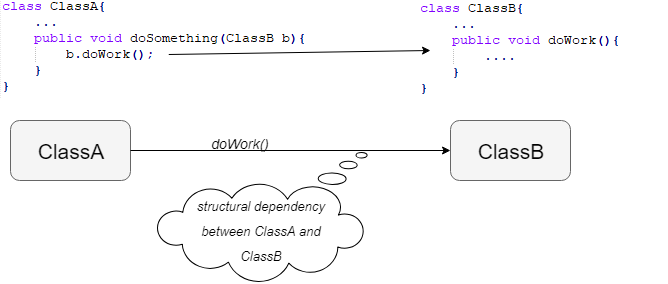
\includegraphics[width=\textwidth]{structural_dep.png}
	\caption{\label{fig:fig}Example of structural dependency between two classes}
     \end{figure}
\end{center}

\end{frame}

%%%%%%%%%%%%%%%%%%%%%%%%%%%%%%%%%%%%%%%%%%%

 \begin{frame}
\frametitle{Logical dependencies}
\begin{block}{Definition}
 Logical dependencies are the result of software history analysis and can reveal relationships that are not present in the source code code (structural dependencies).
\end{block}

\begin{center}
     \begin{figure}
	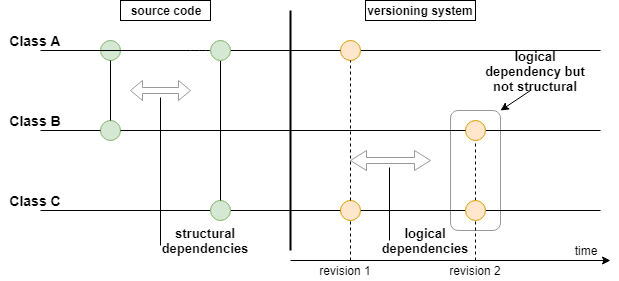
\includegraphics[width=\textwidth]{fig1.png}
	\caption{\label{fig:fig1}Example of logical and structural dependencies}
     \end{figure}
\end{center}

\end{frame}

%%%%%%%%%%%%%%%%%%%%%%%%%%%%%%%%%%%%%%%%%%%

 \begin{frame}
\frametitle{Current status of research in identifying logical dependencies}


\end{frame}

%%%%%%%%%%%%%%%%%%%%%%%%%%%%%%%%%%%%%%%%%%%

 \begin{frame}
\frametitle{Applications of software dependencies}


\end{frame}

%%%%%%%%%%%%%%%%%%%%%%%%%%%%%%%%%%%%%%%%%%%

 \begin{frame}
\frametitle{Current status of doctoral research}


\end{frame}

%%%%%%%%%%%%%%%%%%%%%%%%%%%%%%%%%%%%%%%%%%%

 \begin{frame}
\frametitle{Current status of research in identifying logical dependencies}


\end{frame}

%%%%%%%%%%%%%%%%%%%%%%%%%%%%%%%%%%%%%%%%%%%

 \begin{frame}
\frametitle{Proposed research stages: Development of content and tools }

\textbf{Stage 1:} Build tool to extract structural dependencies from code and co-changes from git for a given set of projects.

\textbf{Stage 2:} Find filters for the co-changes extracted, the filters can be the ones already mentioned in previous works or new ones. Establish different thresholds for those filters.

\textbf{Stage 3:} Study the impact of those filters and the corresponding thresholds on the remaining quantity of co-changes for each system.
Study the overlapping between the remaining pairs of co-changing entities and the structural dependencies extracted \cite{enase19}. 



\end{frame}

%%%%%%%%%%%%%%%%%%%%%%%%%%%%%%%%%%%%%%%%%%%

 \begin{frame}
\frametitle{Proposed research stages: Development of content and tools }

\textbf{Stage 4:} Establish a dynamic way to determine the thresholds for filters in order to fit the best each studied system. Main focus on the threshold for number of occurrences of co-changing pairs.
Use plots or other visual instruments in order to see the highest and the lowest rates for the numbers of occurrences among co-changing pairs.
Also filter those rates into normal and abnormal ones and study what was the cause of the highest rates (code or human related).

\textbf{Stage 5:} Take into account also structural dependencies from all the revisions of the system to filter out the old, out-of-date logical dependencies. 
Study how this affects the remaining number of logical dependencies.Here an extra check is needed, it can be a case in which old structural dependencies that were also logically linked to continue to be logically linked
even after the structural dependency was removed.

\end{frame}

%%%%%%%%%%%%%%%%%%%%%%%%%%%%%%%%%%%%%%%%%%%

 \begin{frame}
\frametitle{Proposed research stages: Usage }

\textbf{Stage 6:} Export the remaining co-changes whom at this step we can call logical dependencies and use them among structural dependencies in tools for architectural reconstruction to evaluate the improvement.

\textbf{Stage 7:} Compare the number of logical dependencies with metrics like Fan Out, Fan In, Efferent Coupling (Ce), Afferent Coupling (Ca) and study their connections.

\textbf{Stage 8:} Identify other tools that use structural dependencies and evaluate the impact of co-changes filtering into logical dependencies for them.

\end{frame}

%%%%%%%%%%%%%%%%%%%%%%%%%%%%%%%%%%%%%%%%%%%

 \begin{frame}
\frametitle{ Scientific reports and deadlines of stages}

\begin{figure}[H]
\centering
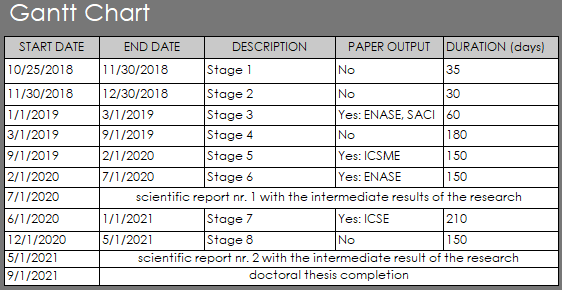
\includegraphics[width=\textwidth]{gantt_chart.PNG}
\label{fig:gantt1}
\end{figure}

\end{frame}


%%%%%%%%%%%%%%%%%%%%%%%%%%%%%%%%%%%%%%%%%%%

 \begin{frame}
\frametitle{Gantt chart}

\begin{figure}[H]
\centering
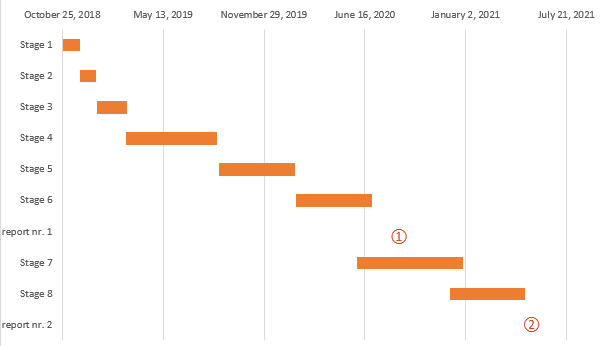
\includegraphics[width=\textwidth]{gantt_plot.PNG}
\label{fig:gantt2}
\end{figure}

\end{frame}


\end{document}